\chapter{Theoretical Framework for Code Refactoring}

\section{Background}
\label{sec:background}

% ---
% Defining Refactoring
% ---

% Intro
Refactoring is a well established concept in software development.
Especially in complex projects, 
	tasks like cleaning and restructuring code are regularly occurring and often times necessary. 
When referring to these activities by name, many employees use the term refactoring. 
The exact definition of the term \emph{refactoring} is not always self-evident,
	despite its familiarity.
To avoid referring to the term too loosely, 
	it is consequently important to give a precise definition as a reference for the following parts of the  thesis. 

% Fowler Refactoring Definition
Martin \textcite{fowler2018} managed to formulate a definition that is both short and precise. 
He is one of the most prominent figures in the field of refactoring, 
	and has pioneered many concepts and ideas, which are also discussed throughout this thesis.
Fowler defines refactoring in the following:
\begin{quote}
\textbf{Refactoring} is the process of changing a software system in a way 
	that does not alter the external behavior of the code yet improves its internal structure.
\end{quote}

% --
% Refactoring Example
% --

% ---
% Objective: Explain External behavior and Internal Structure
% TODO: Refer to example
% ---

\clearpage
\section{Benefits: Why should we refactor?}
\label{sec:benefits}

% Adding Features is attractive
The benefit of refactoring is not as obvious as other activities in software development. 
Spending valuable resources on a process that does not add new functionality 
	might sound unappealing to many managers and software engineers.
Likewise, \textcite{kim2012} discuss the problem of not sensing an immediate benefit when refactoring.
Furthermore, the value of improving the internal structure of the code is hard to demonstrate to a manager, 
	who is not an expert and even harder to present to a client, who is paying for the work.

Having said that, when refactoring is ignored, more time is not necessarily accessible to programmers. 
\textcite{mens2003} argue that through continuous modifications and adaptations to new requirements, 
	the code becomes increasingly complex and drifts away from the original design.
Hence, by not improving the quality of the software, resources will still need to be spent on software maintenance. Bearing in mind Fowler's Definition of refactoring, 
	we therefore aim to mitigate time spent on tedious maintenance, 
by instead improving attributes of the code beforehand.

% Internal Structure = Improving the Quality Attributes
In particular, refactoring helps to improve the internal quality attributes of the software system (\cite{mens2004}). 
For instance, some refactorings remove code redundancy, 
	some raise the level of abstraction, 
	some enhance the reusability.
\textcite{bass1998} distinguishes
	between two categories of quality attributes. 
The first category observes software attributes at runtime. This includes the performance and the security of the software system. The other category does not consider system runtime, but focuses on the quality of the source code. During refactoring, we are only concerned with the latter. This means that we do not consider software quality with respect to its performance and security. 

% Listing Attributes
During a study on the value of quality attributes on refactoring, 
	\textcite{alkhazi2020} identified 
	six of such quality attributes: 
	Reusability, Flexibility, Understandability, 
	Functionality, Extendibility, and Effectiveness.
As a general principle, refactoring adds value if at least one quality attribute has significantly improved, given that the external behavior was not altered.
Accordingly, to make meaningful evaluations, 
	it must be proven that only the internal structure has changed.
This can be achieved by writing software tests beforehand, to then test whether features remained the same after refactoring (\cite{fowler2018}).
As a result, software tests are a major component when deciding the success of a refactor (for further information, refer to \ref{sec:testing}.


% ---
% Criteria: When should we Refactor
% ---

\section{Criteria: When should we Refactor?}
\label{sec:criteria}

% Critical Perspective
From a business standpoint, there needs to be little explanation, 
	when debating time spent on new features and fixing unresolved bugs.
As discussed earlier, it is significantly harder to persuade refactoring, 
	as there are fewer immediate benefits.
For that reason, one needs to verify the necessity of refactoring
	and compare it to the need of other pending tasks.
For instance, \textcite{fowler2018} points out that if the code works and does not ever need to change, 
	it is fine to leave it alone.
In contrast, he suggests that as soon as someone needs to understand how the code works, 
	and struggles to follow it, one has to do something about it.
Generally speaking, a potential improvement in quality therefore does not warrant refactoring by itself.

% Small Refactors
It is crucial to note that refactoring does not have to be a large and complex undertaking.
Even if there is a demand for it, the refactorings themselves are minor.
\textcite{fowler2018} describes refactoring practices as the application of small behavior-preserving steps, 
	allowing to produce a big change by stringing together a sequence of these behavior-preserving steps ). 
For this reason, refactoring as a principle, 
	can always play a part in software development, 
Therefore, with projects that appear to be qualitatively sufficient, 
	active monitoring of the code quality and continuous improvements 
	through refactorings is still advisable.

% Two Hats
This approach leads to the presumption that these activities can be done in parallel.
However, adding features and refactoring at the same time is not recommended.
The interplay between them can be described making use of an analogy developed by Martin \textcite{fowler2018}. 
He sees software development as wearing two hats, 
	and proposes that time should be distinctively divided between adding functionality and refactoring. 
This means that during refactoring one should not add functionality and vice versa. 
To support his point, 
	Fowler adds that “often the fastest way to add a new feature is to change the code to make it easy to add” (\cite{fowler2018}) 
Conversely, once the code is better structured, 
	time can be efficiently spent on adding new capabilities.

% Planned Refactor
This analogy illustrates nicely that refactoring 
	should be an integral part of software development according to Fowler's standpoint. 
Once this relationship between refactorings and adding features is understood, 
	one can better estimate the timing of each activity.
Even though we learned that refactoring at its best is fairly small, 
	by understanding the precise relationship, 
	we can argue that planned refactoring is not always a mistake.
In more concrete terms, if we agree that better structured code 
	allows us to add features quicker, 
	we can infer that there could be moments where dedicated time spent on refactoring 
	is necessary to get the code base into a better state for new features (\cite{fowler2018}).
As a consequence, doing continuous refactoring might not suffice for larger projects. 

However, there needs to be a note of caution. Specifically, one may assume that for software systems with good internal structure, small refactors suffice. In contrast, in software systems that lack quality, one might think that larger refactorings are required. Although intuitively both assumptions generally make sense, there are exceptions to both cases that are important to keep in mind. 

% Arguments
The first assumption, associated with well-structured software, can be disputed if one of the quality attributes gains significantly in importance. Such a situation alone may justify large efforts of refactoring, necessary to reach the desired state. 
% Argument: Lack of importance
The second assumption, associated with software systems that lack quality, does not hold for modules of the codebase that are not a crucial part of the software system. Here, considering the associated costs, it is hard to make a case for planned refactoring and minor restructuring could suffice.

\section{Challenges: What to watch out?}
\label{sec:challenges}
% Intro
Having a comprehensive understanding of the benefits, scope, and timing of refactoring, 
	it becomes evident that many of the difficulties, are related to planning refactoring rather than its execution.
The complexity of planning become more apparent,
	when working within teams.
Going back to the analogy of the two hats, 
	we assumed that the software development process 
	is conducted by a single person. 
In practice, however, 
	the software development in organizations is typically done within a team. 
 This makes refactoring considerably more difficult,
 	knowing that refactoring and adding new features 
	should be a distinct activity. 
Thus, when a programmer decides to refactor parts of the software system,
	it could inhibit others from working on the software at the same time. 
As a result, 
	it is a challenge to clearly separate 
	which part of the code base is being refactored, 
	and which is added functionality. 
The underlying goal is to reach a state,
	where the separate parts are entirely independent. 
It is important to be aware of this challenge, 
	because otherwise the risk of bugs being introduced becomes much higher. 
As a consequence, 

% Counterintuition
Comprehensively planning refactoring 
	may sound intimidating and time-consuming at first.
\textcite{fowler2018} argues against this belief,
	by suggesting that the whole purpose of refactoring 
	is to speed things up.
Positioning refactoring within the broader scale of the project 
	allows to actively decrease risks and 
    enables to focus on the overall quality of the code base.
Even though refactoring is often done on a small scale,
	its effects can be examined 
	throughout the layers of the software architecture.
This is especially apparent when incrementally improving previously discussed attributes,
	such as Extendibility, Reusability, and Flexibility, 
	which in turn affect the whole state of the project. 

% Conclusion: Competence
In practice, 
	“too little refactoring is far more prevalent than too much” 
	(\cite{fowler2018}).
The suggestion that people should attempt to refactor more often, 
	is, however, much easier said than done.
Besides the mentioned difficulties, 
	refactoring can add considerable value, 
	with the precondition that it is properly carried out.
Carrying out refactorings, however, is not always an easy task, 
	requires education, and most definitely experience.

% --
% Code Smells
% --

\section{Formalization of Code Smells}

% Transition: Relationship between Refactoring and Code Smells
Programmers need to be aware of indications that lead to refactoring.
\textcite{fowler2018} argues that deciding when to start refactoring,
	and when to stop,
	is just as important to refactoring,
	as knowing how to operate the mechanics of it.
Particularly, there is oftentimes no a clear-cut moment requiring refactoring. Instead, there commonly exist 
	indications of issues that can be solved by refactoring.
In practice, 
	these indications are known as \emph{code smells} or \emph{design smells} 
	(\cite{lacerda2020}).
These two terms are distinguished by existing either at a lower level,
	known as the code level, or on a higher level, 
	the design level. 
Hence, 
	depending on the degree of complexity, 
	the smells are named code smell or design smell.
As throughout this work we are not concerned 
	with design decisions of the software system, 
	we will from now on refer to the indications as code smells.

% What is a Code Smell?
The term “smell” is used in reference to an internal software problem
	(\cite{lacerda2020}), 
	which can negatively impact software quality 
	(\cite{sonnleithner2021}). 
One might think that software bugs fall into this category, 
	but this is a false assumption.
Although bugs also negatively impact the state of software, 
	code smells do not necessarily cause the application to break.
Nonetheless, these internal problems may lead to other negative consequences,
	such as “impacting software maintenance and evolution”
	\cite{lacerda2020}.
 
% Illustration
\begin{figure}[htp]
    \centering
    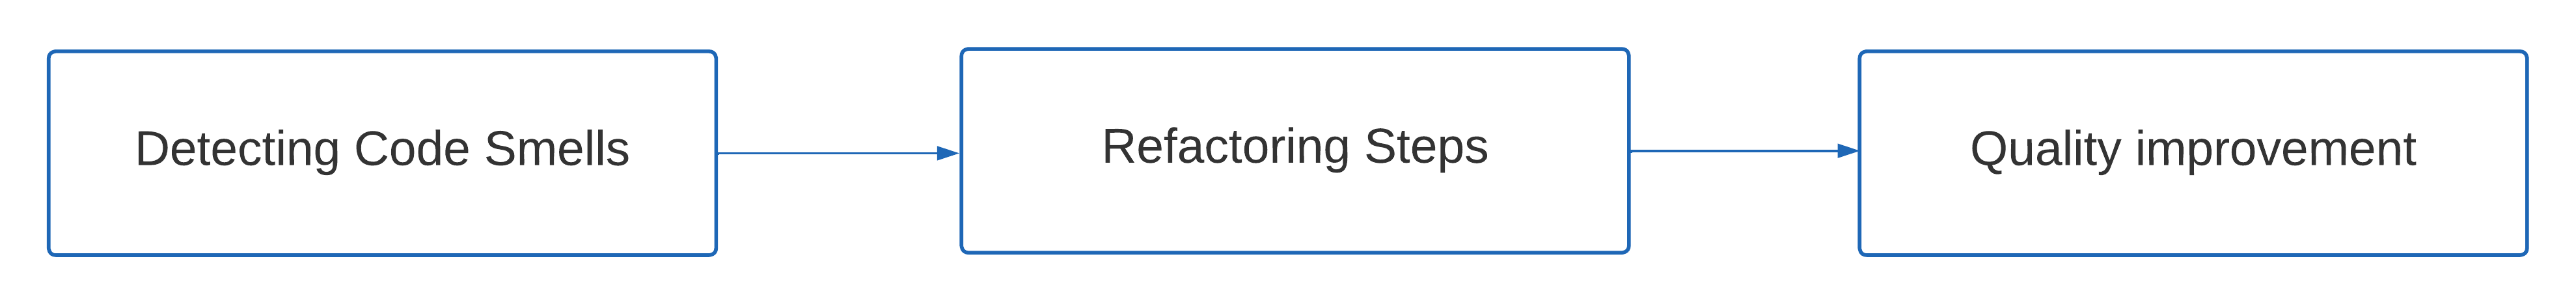
\includegraphics[width=\textwidth]{./assets/simple_process.png}
    \caption{Refactoring process (Simplified Model)}
\end{figure}

% Connection
Knowing that code smells refer to internal problems,
	it becomes apparent that they are closely connected to refactoring, 
	which tries to improve the internal state of the software.
In other words, 
	refactoring can be thought of removing or getting rid of code smells. 

% Examples Intro
To better comprehend the concept of code smells, it is best to list some of them. 
To stay within the scope of this thesis, 
	we will limit the examples to the most prominent ones. 
A selection of ten code smells will be introduced out of 24 code detailed in Fowler's catalog \cite{fowler2018}.
According to a survey conducted by \textcite{lacerda2020}, the following overview briefly summarizes 
	the ten most frequently reported code smells.
\newpage

Summary of code smells identified by Kent Beck and Martin \textcite{fowler2018} 
% Table
\begin{table}[H]
    \centering
\newcolumntype{b}{X}
\newcolumntype{s}{>{\hsize=.5\hsize}X}
\renewcommand{\arraystretch}{1.2}
\scalebox{0.9}{
\label{fig:smells}
\begin{tabularx}{1.2\textwidth}{{sb}}
	Code Smells & Description \\
 \hline
	Duplicated Code & Consists of equal or very similar passages in different fragments of the same code base.  \\
	Large Class & Class that has many responsibilities and therefore contains many variables and methods. \\
	Feature Envy & When a method is more interested in members of other classes than its own,
		is a clear sign that it is in the wrong class \\
	Long Method & A method that is very likely to have too many responsibilities,
		hurting one of the principles of good object oriented design \\
	Long Parameter List & Extensive parameter list, which makes it difficult to understand
		and is usually an indication that the method has too many responsibilities. \\
	Data Clumps & Data structures that always appear together,
		and when one of the items is not present, the whole set loses its meaning \\
	Refused Bequest & Indicates that a subclass does not use inherited data or behaviors \\
	Divergent Change & A single class needs to be changed for many reasons.
		This is a clear indication that it is not sufficiently cohesive and must be divided \\
	Shotgun Surgery & Opposite to Divergent Change,
		because modification requires changing several classes \\
	Lazy Class & Classes that do not have sufficient responsibilities and therefore should not exist \\
\end{tabularx}
}
    \caption{Code Smells Overview}
    \label{tab:my_label}
\end{table}

\chapter{Technical Debt}
\label{sec:Business}

% Introduction
During the lifetime of a project, companies have to inevitably deal with code smells appearing in the software systems. Consequently, associated financial costs can only be mitigated by getting rid of them by refactoring.  A typical example of a common financial cost is the additional work required, when programming with deficient code. Naturally, employees are spending less time when their code is easier to read, understand, and modify. Examining the discussion of the relationship between code smells  and financial costs paves the way to consider refactoring decisions from a business standpoint.

\section{Establish a Business Case}
\label{sec:business-case}
\begin{figure}[H]
    \centering
    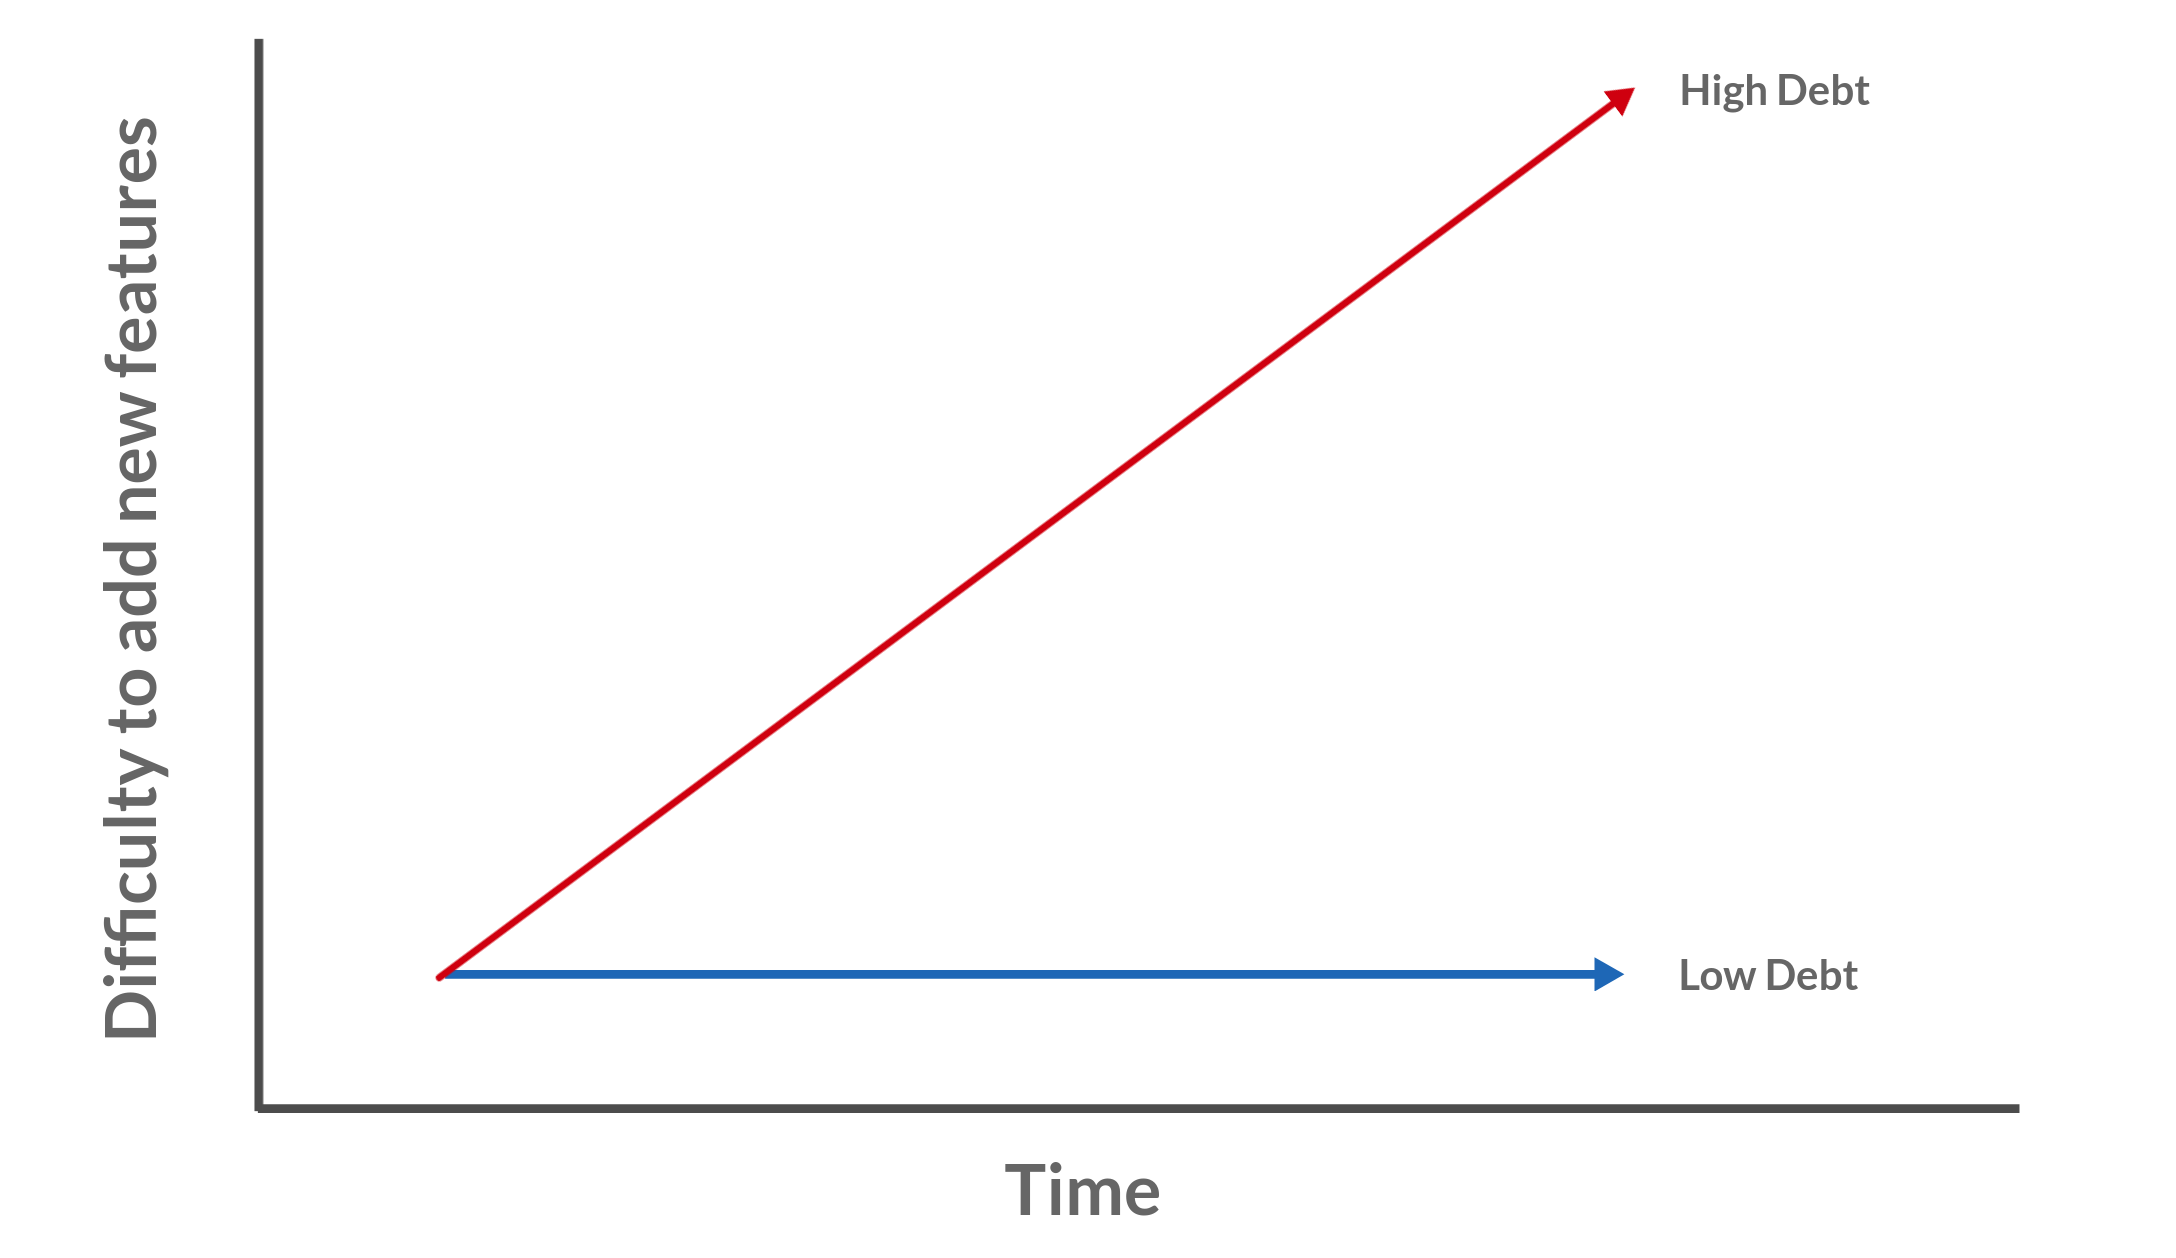
\includegraphics[width=0.6\columnwidth]{./assets/technical_debt}
    \caption{Technical Debt Simplified Depiction}
\end{figure}
% Technical Debt: Explanation
Technical debt is a helpful metaphor 
	that provides a framework that allows thinking about code smells 
	in terms of financial debt (\cite{fowler2019}) in order to establish a firm business case.
In concrete terms, the concept of Technical debt, coined by Ward Cunningham, describes the extra effort it takes to add new features (\cite{kruchten2012}). 
In financial terms, the additional effort is the interest that has to be paid on the accumulated debt (\cite{fowler}). 
Fowler presents the example 
	of a confusing module structure in a code base.
He illustrates that 
	a programmer needs four days to add new features 
	with a clear structure and six days with code smells. 
Then, the two additional days spent is the interest a company has paid on the debt.
We see that a company can either decide to pay the interest on technical debt, 
	or reduce it by means of refactoring. 

% Technical Debt: Unavoidable
One approach to think about solutions is to argue for investing in experienced programmers to avoid debt entirely. 
Based on this assumption, it would sound reasonable to do so, if the additional money spent on the salaries is offset by the cost endured from debt.
In practice, it however is not that simple. Technical debt will always accrue, even with the most experienced of programmers. For instance, technical debt could accumulate solely because one quality attribute gained in importance. It could also be due to the fact that a code base exists for a very long time. In both cases, refactoring is a crucial mechanism in order to get rid of accumulated technical debt. 

% Paradox
Consequently, it becomes apparent, that businesses have financial incentives to make the right decisions in order to efficiently allocate their resources.
There can be instances where technical debt is substantial enough, 
	where associated interest payments can not be handled. 
In some cases, it might be more cost-effective to 
	rewrite an entire code bases instead of refactoring it.  
Difficult decisions require 
	competent employees that are able to decide in ways to deal with the debt. 
These employees are not limited to one type of job role.
Relevant expertise in both management or software engineering department can lead to substantial financial opportunities.


\section{Justify Economic Decisions}
\label{sec:economic-decisions}
% Economic Context
Being aware of the financial relationship, 
	it was just indicated that refactoring must not be restricted to programmers and can also be relevant to managerial roles such as team leaders, or product managers.
Having knowledge of abstract concepts, like technical debt,
	allows employees to participate in decisions and communicate them, without deep knowledge of software engineering.
Instead of relying on best practices in software development, employees are able to offer an evaluation that can be defended from a business standpoint.
Moreover, some might even argue that decisions regarding refactoring should be purely economic. \textcite{fowler2018} claims 
	that it is beneficial to have this attitude and argues that economic benefits
	should always be the driving factor of refactoring.

% Communication Device
Technical debt can a useful device to communicate decision relating to refactoring.
It is a simple model to form significant and potentially complex economic decisions.
The device can be used in two directions, top-down or bottom-up.
In top-down communication, using the term technical debt, provides directions to team members.
As an example, management has decided to migrate their parts of their systems to the cloud, 
	but it team leaders have realized that the code contains a lot of code smells, 
	making it hard to undergo such a change. 
Communicating this issue using the concept of technical debt prevents refactoring parts of code 
	that does not directly contribute to the objective of migration.

% Bottom-up
Likewise, technical debt as a metaphor 
	can also support bottom-up communication.
This metaphor can be used to provide sufficient arguments for refactoring, 
	when clients or upper management are in doubt of such a decision.
For instance, it could serve as a device to reason about 
	the difficulties of adding new features or 
	the issues of making major changes to the application. 
Overall, independent of the direction of communication, knowing technical debt allows companies to have less friction between
	software engineers and its other departments. 